\cotefile{79}
\scanpage{265}
\mspage{135}

En résumé :

\[
\left\{\begin{aligned}
& T_0\ \text{opère fidèlement sur }H,\ \text{et via cette}\\
&\text{opération s'identifie au sous-groupe }\inserted{\widetilde Z}\ \text{de }\operatorname{Aut}(H)\\
&\text{formé des }\bar g\in\operatorname{Aut} H\ \text{satisfaisant les conditions}\\
&\qquad\left\{\begin{aligned}
&\bar g\ \text{normalise }U_0\ \text{et centralise }T_H\\
&\bar g(\sigma)\in\sigma T_H.
\end{aligned}\right.\\
&\text{De plus, on aura alors}\\
&\qquad\bar g(\sigma)=\sigma\,u(\underset{\substack{\shortparallel\\c(\widetilde\delta(g))}}{\underbrace{\delta(g)}}).
\end{aligned}\right.
\tag*{(144)}
\]

% slanted
\margin{\uline{NB} Ces conditions impliquent aussi que $\bar g$ normalise $U_1$ -- en fait, si $\bar g$ \deleted{applique} applique $\sigma T_H=T_H\sigma$ dans lui-\unsure{m\textsuperscript{m}}, alors il normalise $U_0$ ssi il normalise $U_1$.}

En d'autres termes, \deleted{si on désigne par $\widetilde Z$ une ``copie conforme'' de $T_0\subset\operatorname{Aut}(H)$, via $u_0:\widetilde Z\xrightarrow{\sim}T_0$ et $\widetilde\delta_{\!T_0}\deleted{\unsure{u_0}}\unsure{p_0}:T_0\xrightarrow{\sim}\widetilde Z$} alors l'hom $c:\widetilde Z\longrightarrow Z$ s'identifie à l'hom

\[
\deleted{T_0}\widetilde Z\xrightarrow{c_0}T_H\tag*{(145)}
\]

défini par

\[
\bar g\unsure{{}_0|{}}(\sigma)=\sigma\,c_0(\bar g).
\]

i.e on a commutativité dans

\diagram{\makebox[0pt][r]{$(145')$\quad}\begin{tikzcd}[ampersand replacement=\&,column sep=large]
\widetilde Z \arrow[r,"c"] \arrow[dr,"c_0"] \arrow[d,"\deleted{u_0}"'] \& Z \arrow[d,"u","{\unsure{?|\sim|\wr}}"']\\
\deleted{T_0} \arrow[r,"\deleted{\unsure{c_0}}"'] \& T_H
\end{tikzcd}}

Notons d'autre part que l'hom

\[
\begin{aligned}
T_H&\longrightarrow\operatorname{Aut}(H)\\
t&\longmapsto\operatorname{int}_H(t)
\end{aligned}
\]

se factorise visiblement par $\deleted{T_0}\widetilde Z$, et donne un homomorphisme

\[
T_H\xrightarrow{c'_0}\deleted{T_0}\widetilde Z\tag*{(146)}
\]

satisfaisant

\[
c_0(c'_0(t))=t^{-2}\tag*{\deleted{\unsure{(}}(147)}
\]

puisque pour $t\in T_H$, on a

\[
\sigma t\underset{\sigma}{\underbrace{\sigma^{-1}}}=t^{-1}\quad\deleted{\unsure{\text{d'où}}}\ \text{i.e.}\quad t\sigma t^{-1}=\sigma t^{-2},
\]

ce qui suggère qu'on a commutativité dans
% archive sheet number: 264
\scanpage{266}


\diagram{\makebox[0pt][r]{$(148)$\quad}\begin{tikzcd}[ampersand replacement=\&,column sep=large]
\widetilde Z \& Z \arrow[l,"c'"'] \arrow[d,"u\,{\unsure{?|\sim|\wr}}"']\\
\deleted{T_0}\arrow[u,"\deleted{u_0}"'] \& T_H\arrow[ul,"\unsure{c'_0}"]\arrow[l,"\deleted{\unsure{c'_0}}"]
\end{tikzcd}}

\[
\operatorname{int}_H(t^{-1})=c'_0(t^{-1})\longleftarrow\joinrel\shortmid\ t
\]

i.e. qu'on doit avoir

\[
\operatorname{int}_H(u(\lambda))^{-1}\deleted{\unsure{\vert_H}\,\unsure{\operatorname{int}}}
=\operatorname{int}\bigl(u_0(c'(\lambda))\bigr)|H
\]

ou encore

\[
u(\lambda)^{-1}\equiv u_0(c'(\lambda))\quad\bmod\ \operatorname{Cent}_G(H)
\]

\deleted{\unsure{ou on a|i.e. que}}\inserted{i.e. que}

\[
u(\lambda).u_0(c'(\lambda))\in\operatorname{Cent}_G(H)
\]

or on a (128)

\[
u(\lambda)\,u_0(c'(\lambda))=\lambda\unsure{\in|+}Z\in\operatorname{Cent}(G),
\]

ce qui \deleted{\unsure{vient}} prouve (148).

Cela achève donc d'expliciter ce qu'il fallait via $T_0$. On aurait l'explicitation symétrique via $T_1$, avec $U_1$ remplaçant $U_0$ -- mais \inserted{en fait on trouve \uline{le même} sous-groupe de $\operatorname{Aut}(H)$ en fait} \deleted{en passant à $T_G$, on fera attention que $T_G$ n'opère \uline{pas} \uline{fidèlement} sur $H$, donc $T_G$ ne peut s'expliciter comme sous-groupe de $\operatorname{Aut} H$.}

\[
\begin{aligned}
\widetilde Z &=\operatorname{Im}(T_0\to\operatorname{Aut}(H))=\operatorname{Im}(T_1\to\operatorname{Aut}(H))\deleted{\unsure{=\operatorname{Im}(T)}}\\
&=\operatorname{Im}(T_G\to\operatorname{Aut} H)
\end{aligned}\tag*{(149)}
\]

\deleted{Mais} Explicitons encore le sous-groupe $\unsure{\mathfrak z|\mathcal Z}\inserted{=\operatorname{Ker}(\delta_{T_0}:T_0\to Z)}$ de $T_0$ en tant que sous-groupe de $\operatorname{Aut} H$, on trouve \unsure{p}

\[
\begin{aligned}
\mathfrak z&\xrightarrow{\sim}\quad\text{sous-groupe de }\operatorname{Aut}H\ \text{formé des}\\
z&\longmapsto\operatorname{int}(z)|H\quad \text{autom }\bar g\ \text{qui normalisent }U_0,\\
&\hspace{8em}\text{et qui centralisent }T_H\ \text{et }\sigma.\\
&\hspace{8em}\deleted{\text{(donc aussi }\sigma(U_0)\text{)}}\ \text{qui}
\end{aligned}\tag*{(149)}
\]
% archive sheet number: 265
\scanpage{267}
\mspage{136}

\uline{NB} Introduisons

\[
N_H=T_H\cup(\overbrace{T_H\sigma=\sigma T_H}^{\unsure{\Pi|\pi}=T_H\sigma=\sigma T_H})\tag*{(150}
\]

qui est un sous-groupe de $\deleted{\unsure{G}}H$ \deleted{\unsure{normalis|normalisant}} contenant $T_H$ et le normalisant, avec $T_H$ d'indice 2 dans $N$, ou égal à $N$ dans le cas $\sigma\in T_H$, \deleted{d'un} cas \inserted{\unsure{visiblement rare|visiblement cas}} que nous allons écarter pour le moment (cas ``non dégénéré'') :

\[
1\longrightarrow T_H\longrightarrow N_H\longrightarrow\{\pm1\}\longrightarrow1
\qquad\text{si }\sigma\notin T_H\tag*{(151)}
\]

On a donc

\[
\widetilde Z=\left\{\bar g\in\operatorname{Aut}(H)\ \middle|\
\begin{aligned}
&g\ \deleted{\unsure{\text{normalise}}}\text{centralise }\deleted{N}T_H\ \text{et }\deleted{\text{centralise}}\inserted{\text{normalise}}\ \deleted{\unsure{T}}N_H\\
&g\ \text{normalise }U_0\ \text{(ou aussi : }U_1\text{)}
\end{aligned}\right\}\tag*{(152)}
\]

Donc $\widetilde Z$ opère sur la classe $\Pi=\sigma T_H=T_H\sigma$ par translations, via l'hom $c:\widetilde Z\unsure{\longrightarrow|\text{---}}Z$ justement.

\deleted{Le cas ``dégénéré'' s'explicite ainsi}

\deleted{Conditions équivalentes :}

\[
\deleted{\left\{\begin{aligned}
&\text{a) }\unsure{\Phi_0|\$_0|t_0}=S_0\\
&\text{b) }A_0\ \text{est formé des parties ponctuelles de }S\\
&\text{c) }\sigma=1\\
&\deleted{\unsure{\text{d) }\sigma=1}}\\
&\text{d) }\sigma\in T_H\quad\text{i.e. }T_H=N_H\\
&\deleted{\unsure{\text{e) }S\text{ est un torseur sous }H}}
\end{aligned}\right.}\tag*{\deleted{(153)}}
\]

\deleted{Sous \deleted{\unsure{d)}} ces conditions on a $U_0=U_1=\{1\}$, \deleted{et} $S$ est un torseur sous $H$, et $T_H$ est un sous-groupe commutatif tel que $t\in T_H\Rightarrow t^{2}=1$, \inserted{enfin} $\widetilde Z=\operatorname{Cent}_H(Z)$.}

Il y a lieu d'introduire aussi

\[
N_G=T_G\unsure{\cup|+}(\sigma T_G=T_G\sigma)\tag*{(153)}
\]

on a donc, dans le cas où $\sigma\ne1$ (cas non dégénéré)

\[
1\longrightarrow T_G\longrightarrow N_G\longrightarrow\{\pm1\}\longrightarrow1
\qquad\text{si }\sigma\notin T_H\tag*{(154)}
\]
% archive sheet number: 266
\scanpage{268}


Pour le cas ``dégénéré'', notons

\[
\begin{aligned}
\sigma\in T_H&\Longrightarrow U_0=U_1=\{1\},\quad \deleted{\widetilde Z}\ T_H\ \text{un }\deleted{\text{sous-}}\text{groupe}\\
\Updownarrow&\hspace{15em}\text{commutatif avec}\\
\deleted{\unsure{\exists\lambda\in Z,\ t_0=\lambda s_0}}&\hspace{15em}t\in T_H\longrightarrow t^2=1\\
t_0\in Z.s_0&\qquad\text{enfin }\widetilde Z=\operatorname{Cent}_H(T_H).\\
\text{i.e. }\underset{D_0}{\underbrace{t_0^{\unsure{\leftrightarrows|\leftrightarrow|\Diamond}}}}
=\underset{D_1}{\underbrace{s_0^{\leftrightarrows}}}&
\end{aligned}\tag*{(155)}
\]

% slanted
\margin{\unsure{implique|impliques} donc que $S$ est un \uline{torseur} sous $H$ ($\Longleftrightarrow U_0=\{1\}\Longrightarrow U_1=\{1\}$),}

\deleted{\unsure{ainsi} Notons que la} Plus précisément, la donnée d'un multigraphe à homothéties et groupe simplement transitif d'autom \inserted{et \deleted{point} épinglé par $(\unsure{a|s|s_0},b)\in A_0$,} \deleted{tel que $\sigma\in T_H$ i.e} et tel que $s_0^{\leftrightarrows}=t_0^{\leftrightarrows}$ i.e $\sigma\in T_H$, \uline{équivaut} à la donnée de $H$, du sous-groupe commutatif $T_H$ tel que $T_H^2=\{1\}$, et de $\sigma\in T_H$ -- et on aura alors $\widetilde Z=\operatorname{Cent}_H(T_H)$.

\deleted{Considérons}\inserted{Notons} le cas, encore plus dégénéré

\[
\sigma=1\ .\Longleftrightarrow s_0=t_0\Longleftrightarrow
\begin{aligned}& A_0\ \text{est formé des parties}\\[-2pt]&\text{ponctuelles de }S.\end{aligned}\tag*{(156)}
\]

\begin{center}\rule{2.1cm}{0.3pt}\end{center}

\unsure{1} Digression dans le cas d'un multigraphe avec \inserted{gr de} homothéties \inserted{$Z$}, et groupe \deleted{d'}\inserted{de $Z$-}autom. $H$ simplement transitif sur \deleted{les arêtes} un des $\overrightarrow A_\lambda$ (donc sur tous) -- Fixons nous une origine $s_0$ et un rayon incident \unsure{à|:} $s_0$

\[
\deleted{\unsure{s_0,\ \text{donc}|\text{donc }s_0}}\quad s_0\in S,\ D_1\in S^{\leftrightarrows},\quad D_0=Z.s_0\ \text{et }D_1\ \text{incidents dans }S^{\leftrightarrows}\ ;\tag*{(157)}
\]

donc on a

\[
\begin{aligned}
S&\simeq H/U_0\qquad\text{où}\quad U=H_{s_0}\\
&\text{(isom de }H\text{-ensembles)}\ ,
\end{aligned}\tag*{(158)}
\]

\deleted{fixons nous en plus un rayon} de plus $T_G$, $T_0$ \deleted{\unsure{G_{\leftrightarrows}} et} $G_S$ sont bien déterminés par (137), \deleted{et $N_1$} ou (90) (\unsure{93|92|97}), donc aussi $T_H=T_G\cap H$ :

\[
\deleted{T_H\subset H,\ T_0\subset T_G\in G,}
\]
% archive sheet number: 267
\scanpage{269}
\mspage{137}

\diagram{\makebox[0pt][r]{$(159)$\qquad}\begin{tikzcd}[ampersand replacement=\&,row sep=small,column sep=small]
\& \unsure{e|\mathrm e}\arrow[r,hook,no head]\arrow[d,hook,no head] \& U_0\arrow[d,hook,no head]\\
\& T_H\arrow[r,hook,no head]\arrow[d,hook,no head] \& H\arrow[d,hook,no head]\\
T_0\arrow[r,hook,no head] \& T_G\arrow[r,hook,no head] \& G
\end{tikzcd}\ .}

Bien sûr, $\sigma$ n'est pas déterminé en termes des données précédentes, mais on a

\[
\left\{\begin{aligned}
N_{\deleted{H}G}&=\{g\in\deleted{H}G\mid u(\{D_0,D_1\})=\{D_0,D_1\}\},\quad\text{d'où}\\
&\deleted{\text{donc }N_H\unsure{=}}\\
N_H&=N_G\cap H=\{g\in H\mid u(\{D_0,D_1\})=\{D_0,D_1\}
\end{aligned}\right.\tag*{(160)}
\]

l'hom

\[
N_G\longrightarrow\{\pm1\}\qquad
\begin{aligned}&(\text{si }\sigma\notin H\unsure{\}},\text{ i.e.}\\&D_0\ne D_1)\end{aligned}
\]

étant donné par l'action de $g$ sur la paire $D_0,D_1$ \ldots. Ainsi $N_G$, $N_H$ et l'hom $N_G\to\pm1$ \deleted{de} de noyau $T_G$ (resp. $N_H\to\pm1$ de noyau $T_H$) sont déterminés par les données. Ceci dit, on a des \deleted{bijections}\inserted{isom} canoniques de $Z$-torseurs

\[
\begin{aligned}
&\deleted{\unsure{D_1\xrightarrow{\sim}\Pi}\ \unsure{\xrightarrow{\sim}}}\quad
\underset{\substack{\deleted{\unsure{N_H\setminus H}}\\\text{image inverse de }-1\\\text{par }N_H\to\{\pm1\}}}{\underbrace{N_H^-}}\xrightarrow{\sim}D_1\xrightarrow{\sim}\unsure{\Pi|\pi}\\
&\deleted{t_0\mapsto\unsure{\tau}(s_0,t_0)}\hspace{5em}
\sigma\longmapsto\sigma(s_0),\ t_0\longmapsto\tau(s_0,t_0)
\end{aligned}\tag*{(\unsure{151|161})}
\]

\deleted{l'isom} \deleted{obtenu par} où on prend sur $N_H^-$ la structure de $Z$ torseur \unsure{défini|définie} par les opérations \uline{droites} de $T_H\xleftarrow[u]{\sim}Z$ sur $N_H^-$, i.e. \deleted{\unsure{$\lambda$}}

\[
\lambda\in Z\ \text{opère sur }N_H^-\ \text{par}\quad g\longmapsto gu(\lambda).\tag*{(162)}
\]

Notons ici :
% archive sheet number: 268
\scanpage{270}


(163)\quad Il y a une \deleted{\unsure{équivalence|détermination}}\inserted{équivalence} entre les données $(S,H,Z,\unsure{\Pi|\pi},s_0,D_1)$ d'un multigraphe à homothéties avec groupe de \inserted{$Z$-}autom $H$ \inserted{simplem.} transitif sur les $\overrightarrow A_\lambda$, un sommet marqué $s_0$ et un rayon $D_1$ incident à $Zs_0=D_0$ marqué, \inserted{avec $D_0\ne D_1$ ($\Leftrightarrow$ cas ``non dégénéré'')} d'une part,

et d'autre part : les systèmes $(H,U_0,T_H,N_H)$ d'un groupe $H$, et de ss-groupes $U_0,T_H,N_H$, satisfaisant :

a) $T_H$ normalise $U_0$, et $T_H\cap U_0=\{1\}$ (d'où produit 1/2 direct $B_H=T_H.U_0$)

b) $N_H\supset\deleted{\unsure{B_H}}T_H$, $T_H$ d'indice \deleted{\illegible{1}} 2 dans $N_H$ (qui normalise donc $T_H$) -- de sorte que les $\sigma(U_0)$ pour $\sigma\in N_H\setminus T_H\inserted{=N_H^-}$ \inserted{sont} tous égaux à un \unsure{m\textsuperscript{me}|même} ss-groupe $U_1$ de $H$

c) \deleted{$T_H$ commutatif, et $N_H/T_H$ \unsure{opère} par inversion sur $T_H$ par $t\mapsto t^{-1}$} $\sigma\in N_H^-\Longrightarrow\sigma^2=1$ ($\Rightarrow T_H$ est comm et $N_H/H\simeq\pm1$ y opère par $t\mapsto t^{-1}$)

d) $U_0\cap U_1=\{1\}$ (où $U_1$ défini dans b)).

On aimerait vérifier aussi la formule familière

\[
B_H\cap N_H=T_H\tag*{(164)}
\]

% slanted
\margin{donc la donnée de $(U_0,T_H,N_H)$ équivaut à celle de $(U_0,B_H,N_H)$, d'où on tire en effet $T_H=B_H\cap N_H$ ; \deleted{\unsure{puis}} \deleted{\unsure{et}} Dans certains cas importants, on aura d'ailleurs $U_0=[B_H,B_H]$ (en tous cas $\supset$) et tout est déterminé en termes de $B_H,N_H$ ss-groupes de $H$.}

\unsure{alors que|i.e.} le groupe $B_H\cap N_H$ est compris entre $T_H$ et $N_H$ -- donc si $\sigma\in N_H^-$ est donné, la formule (164) équivaut à

\[
\sigma\notin B_H\tag*{(165)}
\]

Mais si on avait $\sigma\in B_H\deleted{\unsure{=T_H.U_0=T_H|=B_H\,U_0\,T_H}}$, on aurait $\sigma\deleted{\unsure{\in}}(U_0)=\unsure{U_0|U_1}$ \inserted{de par d) $U_0=\{1\}$, donc $B_H=T_H$ donc $\sigma\in T_H$,} absurde.

\deleted{$u\in U_0,\ t\in T_H$, donc (comme $t$ centralise $T_H$, alors que $\sigma=ut$ le renverse et y induit $g\mapsto g^{-1}$) il faudrait que : $u\in U_0$ normalise $T_H$, et y induit $g\mapsto g^{-1}$ comme $T_H$ normalise $U_0$ et $T_H\cap U_0=\{1\}$, cel n'est possible que si $g\in T_H\Rightarrow g^2=1$ i.e \deleted{\unsure{de sorte}} $g=g^{-1}$ ($u$ \uline{centralise} $T_H$). \deleted{et} Donc $B_H\cap N_H=N_H$ i.e. $N_H\subset B_H$, \inserted{et alors}}

\[
\deleted{\left.\begin{aligned}
&\text{On a ou bien (164), \uline{ou} \uline{bien} }\quad T_H^2=\{1\}\ \text{et}\\
&N_H=\{1,u_0\}\times T_H,\ \text{où }u_0\in U_0\ \text{est un élément d'ordre }2\\
&\hspace{5em}\text{qui centralise }T_H,\ \text{i.e. }u_0\in{}_2(U_0^{T_H}),u_0\ne1.
\end{aligned}\right.}\tag*{\deleted{(165)}}
\]
% archive sheet number: 269
\scanpage{271}
\mspage{138}

4. Cas des graphes triangulants.

Un graphe $(S,A_0)$ \inserted{sans boucles \deleted{isolés}} est dit \uline{triangulant} si

\[
\begin{aligned}
&\forall\,s,t\in S,\ \text{tels }\deleted{\unsure{\exists}}\text{que }\{s,t\}\in A_0,\quad
\exists\,u\in S\ \text{tel que }\{s,u\},\{t,u\}\in A_0\\
&\hspace{13em}\text{i.e tel que }\{s,t,u\}\in F_0
\end{aligned}\tag*{(1)}
\]

où on a posé

\[
F_0=\{f\in\unsure{\mathfrak P_3(S)|P_3(S)}\mid\forall\,a\in\mathfrak P_2(f),\ \text{on a }a\in A_0\}.\tag*{(2)}
\]

\deleted{La condition d'homogénéité \unsure{conve|comm}}
Lorsqu'on est en présence d'un \uline{multigraphe} à homothéties \deleted{de} $Z$, on dit qu'il est triangulant si chacune des structures de graphe est triangulante. Il suffit \inserted{pour ceci,} lorsque les \deleted{\unsure{ces}} structures sont isomorphes entre elles (``condition d'isomorphie'' du § 2) que l'une d'elles soit triangulante. \deleted{\unsure{4}} Mais il n'est \deleted{pas} sans doute pas vrai qu'il en soit ainsi dans tous les cas.
% archive sheet number: 270
\scanpage{273}


\diagram{\small\(\begin{array}{l|c||c|c|c|}
\hfill n & 2 & 3 & 4 & 5\\\hline
[\operatorname{Sl}(2,\mathbb Z/n\mathbb Z)]&6&24&48&120\\\hline
[\operatorname{Gl}(2,\mathbb Z/n\mathbb Z)]&6&48&96&480\\\hline
[\operatorname{Sl}(2,\mathbb Z/n\mathbb Z)']&6&12&24&60\\\hline
\operatorname{Sl}(2,\mathbb Z/n\mathbb Z)'&\unsure{\mathfrak S_3|\mathcal G_3}=D_3&\mathfrak S_4^+&\mathfrak S_4&\mathfrak S_5^+\\\hline
[\operatorname{GP}(1,\mathbb Z/n\mathbb Z)]&6&24&48&120\\\hline
\operatorname{GP}(1,\mathbb Z/n\mathbb Z)&\mathfrak S_3=D_3&\mathfrak S_4&\mathfrak S_4\times\{\pm1\}\,?&\mathfrak S_5\,?\\\hline
[M^*]&3&8&12&24\\\hline
[\overbrace{M^*/\{\pm1\}}^{S_M}]&3&4&6&12\\\hline
\text{type }M^*/\{\pm1\}&\deleted{\unsure{\text{té}}}\unsure{\text{triangle}|\text{trièdre}}&\text{tétraèdre}&\text{octaèdre}&\text{icosaèdre}\\\hline
[P(M)]&3&4&6&6\\\hline
[F_M^{\unsure{\infty|a|*}}]\deleted{\unsure{/\{\pm1\}}}&1&\deleted{\unsure{4}}\,\unsure{8|1|4}&\deleted{\unsure{8}}\,\unsure{16|8}&\deleted{\unsure{2}}40\\\hline
[F_M^0]&1&4&8&20\\\hline
\end{array}\)}

Soit $M$ un module libre de rang 2 sur \illegible{3} \unsure{idéaux|ci-dessus|dérons}
% archive sheet number: 272
\scanpage{274}


\[
(\mathbb Z/n\mathbb Z)^{2\,*}
\]
% archive sheet number: 273
\scanpage{276}


Détermination d'un sommet (d'un \inserted{2-}polyèdre triangulé) par son étoile.

1) Soient $\inserted{P=}(S,F\subset\unsure{\mathfrak P_3(S)|P_3(S)})$ un 2-polyèdre triangulé connexe, $s,s'\in S$ tels que \deleted{\unsure{s}} l'on ait

\[
s\ne s',\quad\operatorname{Et}(s)=\operatorname{Et}(s').
\]

Alors on a

\[
S=\{s,s'\}\cup\operatorname{Et}(s)
\]

i.e. $P$ s'identifie au double cône sur le $n$-polygône $\operatorname{Et}(s)$ ($n\inserted{=\operatorname{card}\operatorname{Et}(s)}\geq3$).

\figure{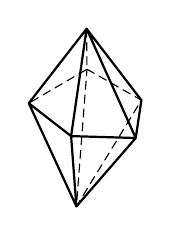
\begin{tikzpicture}[x=.48cm,y=.48cm,line cap=round,line join=round]
\coordinate (N) at (0.22,2.95);\coordinate (S) at (-0.05,-1.75);
\coordinate (L) at (-1.31,.98);\coordinate (F) at (-.19,.11);
\coordinate (R) at (1.52,.06);\coordinate (E) at (1.67,1.06);\coordinate (B) at (.23,1.88);
\draw[thick] (N)--(L)--(F)--(R)--(E)--cycle (N)--(F)--(S)--(R)--(N) (L)--(S);
\draw[densely dashed] (N)--(B)--(L) (B)--(E)--(S)--(B);
\end{tikzpicture}}

\uline{NB} Les deux sommets $s,s'$ sont d'ordre $n$, les autres sommets sont d'ordre 4. Si tous les sommets ont même ordre, on a donc $n=4$, et $P$ est un octaèdre. Dans ce cas, pour que deux sommets aient même étoile, il f. et s. qu'ils soient antipodiques. Dans le cas $n\ne4$, la seule paire de sommets ayant $\unsure{=|\text{m\textsuperscript{me}}}$ étoile est $\{s,s'\}$ (car \deleted{\unsure{que}} s'il y avait une autre \deleted{\unsure{sommet}} telle paire $\{t,t'\}$, \deleted{les} l'ordre de $t,t'$ serait quatre, et $P$ serait un octaèdre, absurde !). Mais dans ce cas, il existe encore un automorphisme unique (qui mérite le nom d'antipodisme ?) \unsure{$u$|$a$|i.e.}\inserted{$\underline a\ne\mathrm{id}$}, tel que pour \deleted{que} $t\in S$, on ait $\operatorname{Et}(t)=\operatorname{Et}(\underline a(t))$ ; cet automorphisme est la transposition de $s,s'$ et l'identité sur $E=\operatorname{Et}(s)=\operatorname{Et}(s')$. Il est involutif, et ses orbites sont les classes pour la relation
% archive sheet number: 275
\scanpage{277}


d'équivalence \deleted{\unsure{entre}}\inserted{des} $\unsure{t|f|S}$

\[
t\sim t'\ \overset{\mathrm{déf}}{\Longleftrightarrow}\ \operatorname{Et}(s)=\operatorname{Et}(t').
\]

Cette dernière propriété est une \deleted{\unsure{con}}caractérisation de $\underline a$ commune à tous les cas (aussi bien $n=4$ que $n\ne4$).

2) Soient $\Lambda$ un anneau semi-local, \deleted{et soient}\inserted{$M$ un} module libre de rang 2 sur $\Lambda$, $u,u'\in M^*$ tels que l'on ait

\[
\left\{\begin{aligned}
&\forall\,x\in M^*,\qquad u\wedge x\in(\det M)^*\ \Longleftrightarrow
\bigl(\deleted{u'\wedge x\in(\det M)^*}\\
&\hspace{14em}\deleted{\Longrightarrow}\inserted{\text{et}}\quad u'\wedge x\in\pm\{u\wedge x\}
\end{aligned}\right.\tag*{$(*)$}
\]

% slanted
\margin{\uline{NB} Le cas exceptionnel est aussi celui où le normalisateur de $\operatorname{Gl}_\Lambda(M)^{\pm}$ dans $\unsure{\mathfrak S_{S_M}|\mathcal G_{S_M}}=\mathfrak S_{(M^*/\pm1)}$ n'est pas réduit au groupe \deleted{\unsure{$Z$}} $\Lambda^*/\pm1$ opérant de façon \unsure{identique|évidente} et par cons, \unsure{l'antipodisme} \unsure{fleurit|fleuris}.}

Alors, on a $u'\in\{\pm u\}$, sauf dans le cas suivant :

\[
\begin{aligned}
&\deleted{\unsure{2_\Lambda\in\Lambda}}\quad 2\Lambda=\{0,2\}\ne\inserted{\{0\}}\deleted{\unsure{\Lambda}}\ \text{i.e.}\\[-2pt]
&\qquad\left\{\begin{aligned}
&\inserted{\Lambda\ \text{une }\mathbb Z/4\mathbb Z\text{-alg.}}\\
&\deleted{\unsure{2_\Lambda\ne0,\ 2_\Lambda\in\operatorname{Nil}(\Lambda)\ \text{et}}}\ \text{extension}\\
&\text{d'une }\mathbb F_2\text{-algèbre }\Lambda_0=\Lambda/2\Lambda\\
&\text{par un idéal de carré nul}\\
&\text{engendré par }2_\Lambda\ \text{et qui est}\\
&\text{de rang }1\ \text{en tant que }\mathbb F_2\text{-}\\
&\text{module [correspondant donc à}\\
&\text{un \uline{caractère} }\chi:\Lambda_0\to\mathbb F_2].
\end{aligned}\right.
\end{aligned}
\]

Notons d'abord

\uline{Lemme} La \deleted{assertion}\inserted{relation} ``$\forall\,x\in M^*\quad u\wedge x\in\det M^*\Longrightarrow u'\wedge x\in\det M^*$'' équivaut à ``$\forall\,\mathfrak m_i\in\operatorname{Max}(\Lambda)$, \deleted{\unsure{soi}} les images $u_i^\circ$ et $ {u'}_i^\circ$ de $u,u'$ dans le corps résiduel $k_i=\Lambda/\mathfrak m_i$ sont \deleted{proportionnelles}\inserted{colinéaires} [\uline{NB} les conditions $u,u'\in M^*$ \deleted{\unsure{qui}} impliquent que $u_i^\circ,{u'}_i^\circ$ sont $\ne0$] -- c'est \inserted{donc} une relation d'\uline{équivalence} entre $u,u'\in M^*$. Cette relation implique l'existence d'une base $e,f$ de $M^*$, telle que l'on ait $u\wedge e,u\wedge f,u'\wedge e,u'\wedge f\in\det M^*$, i.e.

\[
u=ae+bf,\quad u'=a'e+b'f\qquad\text{avec }a,b,a',b'\in\Lambda^*,
\]

et on peut \unsure{$=$} supposer, quitte à remplacer $e,f$ par $ae,bf$, que $\inserted{a=b=1\quad\text{i.e. }u=e+f}$. Si on suppose maintenant $u\wedge x\in\det M^*\Longrightarrow u'\wedge x\in\pm\{u\wedge x\}$, faisant $x=e$, puis $x=f$, on voit que \deleted{\unsure{$a',b'\in\{\pm a\}$|$a'\in\{\pm a\}$}},

\[
a'\in\{\pm1\},\quad b'\in\{\pm1\},
\]

donc quitte à changer $u'$ de signe, ops

\[
u=e+f,\quad u'=e\pm f
\]
% archive sheet number: 276
\scanpage{278}


et il s'agit de voir que l'on \unsure{ne peut|en peut} avoir

\[
u=e+f,\quad u'=e-f
\]

sauf \deleted{dans le cas précisé} si $2\,1_\Lambda=0$, (où on a $\inserted{+1_\Lambda=-1_\Lambda\ \text{donc}}u=u'$, et on gagne), \inserted{ou dans le cas précisé dans l'énoncé ci-dessus.} Supposons donc

\[
2.1_\Lambda\ne0
\]

Notons que \deleted{puisque $u\equiv u'$}\inserted{comme $u_i^\circ,{u'}_i^\circ$} sont colinéaires dans tout corps résiduel $k_i$, cel implique déjà que $2\,1_{k_i}=0$ pour tout $i$, i.e.

\[
2.1_\Lambda\in\unsure{\mathfrak r|\mathfrak R|k}\,\Lambda.
\]

La condition $(*)$ sur $x\in M^*$ s'écrit, écrivant

\[
x=\alpha e+\beta f\qquad\alpha,\beta\in\Lambda
\]

que

\[
\alpha+\beta\in\Lambda^*\ \Longrightarrow\ \deleted{\unsure{2\alpha\ \text{ou}|2\alpha\ \text{ou }2\beta}}\alpha+\beta\in\pm(\alpha-\beta)\quad\text{i.e. }2\alpha\ \text{ou }2\beta\ \text{nul.}
\]

Posant $\lambda=(\alpha+\beta)$ et multipliant $\alpha,\beta$ par $\lambda^{-1}$, on est ramené à voir que

\[
\begin{aligned}
&\alpha,\beta\in\Lambda,\ \alpha+\beta=1\Longrightarrow 2\alpha\ \text{ou }2\beta\ \text{nul }\deleted{\unsure{\text{ce}}},\ \text{i.e.}\\
&\forall\,\alpha\in\Lambda,\ \text{on a }2\alpha\ \text{ou }2(1-\alpha)=2-2\alpha\ \text{nul, i.e.}\\
&\deleted{\unsure{(**)}}\qquad 2\Lambda\subset\{0,2\},\quad\text{donc (puisque }2.1_\Lambda\ne0\text{)}\\
&\deleted{\unsure{(***)}}\qquad \boxed{2\Lambda=\{0,2\}\ne\{0\}},\quad\text{(qui implique }4_\Lambda=0\ \ldots\text{)}
\end{aligned}
\]

\uline{Remarque}

On voit que dans ce cas, les \deleted{couples}\inserted{paires} $\{u,u'\}$ qui mettent en défaut la conclusion escomptée $\{u'\in\pm u\}$ forment une orbite sous $\operatorname{Gl}_\Lambda(M)$, On peut aussi écrire, plus précisément

\[
\begin{aligned}
u'&=u-2f=u+2f\qquad(\text{NB }4_\Lambda=0),\\
(\text{d'où}\quad -u'&=-u-2f=-u+2f)
\end{aligned}
\]

où $2f$ ne dépend que de $f$ modulo l'idéal \inserted{$\mathfrak m_{i_0}$} annulateur de 2, qui est un idéal maximal à corps résiduel \deleted{\unsure{$\mathbb F_2$}}

\[
k_{i_0}\simeq\mathbb F_2
\]

on a \deleted{\unsure{donc}} une suite exacte

\[
0\xrightarrow{\unsure{1|{}}}\underset{\substack{\simeq 2M\\\text{vectoriel de}\\\text{rang 2 sur }k_{i_0}\simeq\mathbb F_2}}{\underbrace{M\otimes_\Lambda k_{i_0}}}\longrightarrow M\longrightarrow M/2M\longrightarrow0
\]
% archive sheet number: 277
\scanpage{279}


Ainsi on peut écrire

\[
u'=u+\unsure{\zeta|\xi}=u-\zeta\qquad(\text{car }2\zeta=0)
\]

où $\zeta$ est un des trois éléments $\ne0$ de $2M\simeq M\otimes_\Lambda k_{i_0}$, et plus précisément, un des deux éléments \deleted{\unsure{$\ne$}}

\[
\zeta\in[(2M=M\otimes_\Lambda k_{i_0})\setminus\{0,2u\}]
\]

(NB $\zeta\notin\{0,2u\}$ signifie justement que $u+\zeta\notin\{\pm u\}$)

Si

\[
2M\setminus\{0,\underset{\unsure{\eta|?}}{\underbrace{2u}}\}=\{\zeta',\zeta''\},
\]

notons que \unsure{l'on a|alors}

\[
\deleted{\unsure{2u}}\underset{2u}{\underbrace{\eta}}+\zeta'+\zeta''=0
\]

donc

\[
u+\zeta'=\underset{-u-\zeta''}{\underbrace{-(u+\zeta'')}}\quad\unsure{\text{i.e.}}
\]

i.e. l'image de $u'$ dans $M^{\unsure{*}}/\{\pm\operatorname{id}_M\}=S_M$ est uniquement déterminée par $u$. \deleted{Ainsi} On \deleted{peut} a ainsi une bijection canonique

\[
\underline a:S_M\longrightarrow S_M
\]

qui associe à tout $\dot u\in S_M$ l'unique $\dot u'\in S_M$ tel que l'on ait

\[
\operatorname{Et}^{\deleted{\unsure{*}}}_{i}(\dot u)=\operatorname{Et}_i(\dot u'),\quad \dot u'\ne\dot u
\]

pour un $i\in\unsure{\Pi_M|\pi_M}=(\det M)^*/\pm1_\Lambda$ -- ce qui est alors vrai pour tous. On voit de suite que $\underline a$ est involutif, \inserted{et} ss pts fixes par construction.

On peut voir \deleted{\unsure{cet|les}}\inserted{décrire} antipodisme par la suite exacte

\[
0\longrightarrow\deleted{\unsure{\operatorname{End}(M_0)}}\underset{\simeq\operatorname{End}_{\mathbb F_2}(M_0)}{\underbrace{\unsure{N|\mathcal N}}}\longrightarrow\operatorname{Aut}_\Lambda(M)\longrightarrow\operatorname{Aut}_{\Lambda/2\Lambda}(M/2M)\longrightarrow1
\]

où $M_0=M\otimes_\Lambda(k_{i_0}\simeq\mathbb F_2)$, et on a

\[
\begin{aligned}
&\operatorname{End}(M_0)\simeq M_0\oplus\mathbb F_2^{\unsure{\underline\omega_J|\omega_J|\simeq J}}\qquad(J=M_0^*),\\
\text{Donc}\quad&\deleted{\unsure{\operatorname{End}(M_0)}}N/\{\pm\operatorname{id}_M\}\simeq M_0\oplus\mathbb F_2^{\underline\omega_J}/\text{diag}\simeq M_0+\mathbb F_2
\end{aligned}
\]

et l'élément non nul du facteur $\mathbb F_2$ donne $\underline a$.
% archive sheet number: 278
\scanpage{280}


Le \deleted{\unsure{cas}} cas le plus simple est celui où

\[
\Lambda=\mathbb Z/4\mathbb Z
\]

c'est aussi celui où $(\unsure{S_M|A_M},F_M)$ est justement l'octaèdre, dont on retrouve l'antipodisme par \deleted{voie} d'algèbre linéaire. La construction \inserted{\unsure{précédente|particulier}} de l'antipodisme est évidemment indépendante de l'hyp. \unsure{semi-locle|semi-locale} sur $\Lambda$, elle marche dès qu'on a $2\Lambda=\{0,2\}\ne\{0\}$, et dans $S_M$ on aura encore

\[
\left\{\begin{aligned}
&\operatorname{Et}_{\deleted{\unsure{u}}i}(u)=\operatorname{Et}_i(\underline a(u))\qquad\forall\,u\in S_M,\ i\in\unsure{\Pi_M|\pi_M}\\
&\underline a(u)\ne u
\end{aligned}\right.
\]

-- mais il n'est pas vrai nécessairement qu'il n'y a pas d'autres éléments que $u,u'\inserted{=\underline a(u)}$ ayant $\unsure{=|\text{m\textsuperscript{me}}}$ étoile que $u$ \ldots\ \deleted{Le cas dé}

\uline{NB} Dans tous les cas, on a

\[
\underline a\in\operatorname{Gl}'_\Lambda(M)^{\pm}
\]

car comme

\[
\underline a\equiv\mathrm{id}\quad\bmod 2\Lambda=\{0,2\unsure{]|\}},\quad\text{on a}
\]

\[
\det\underline a\in1+\{0,2\}=\{\pm1\}.
\]

En fait, on vérifie que

\[
\det\underline a=-1
\]

(car les éléments de $\unsure{N|\mathcal N}$ qui sont dans $\operatorname{Sl}_\Lambda(M)$ sont ceux de $\operatorname{Im}(M_0\oplus\mathbb F_2\,\mathrm{id})$, et $\underline a\in N\simeq\operatorname{End}_{\mathbb F_2}(M_0)$ n'est pas dans ce sous-module \ldots
% archive sheet number: 279
\scanpage{281}
% archive sheet number: 280

\[
\left\{\begin{aligned}
1)\quad &\{\deleted{\unsure{x}}s,\deleted{\unsure{y}}t\}\in A_{\unsure{q|0}},\ \deleted{\unsure{u\in S}}\quad\Longrightarrow\quad
\deleted{\exists}\ \text{il existe exactement deux}\\
&\hspace{14em}\text{éléments }\deleted{\unsure{2u}}\ \text{tels que}\\
&\hspace{14em}\{\deleted{\unsure{x}}s,u\}\ \text{et }\{\deleted{\unsure{y}}t,u\}\in A_0\\
&\deleted{\unsure{\{x,y|\{s,t\}}}\\
2)\quad &\forall\,\deleted{\unsure{x}}s,\deleted{\unsure{y}}t\in S,\ \exists\,u\in S\ \text{tel que}\quad\{s,u\},\{t,u\}\in A\\
&\hspace{8em}\text{et OPS }\{s,u\}\in A_0
\end{aligned}\right.
\]

\deleted{\uline{Corollaire}}\qquad \uline{Corollaire} $\forall\,s,t\in S$, $\exists\,u,v,w\in S$ tels que $(s,u,v,\deleted{\unsure{w}},t)$ soit une $A_0$ chaine.

\diagram{\begin{tikzcd}[ampersand replacement=\&,column sep=small,row sep=small]
s\arrow[dr,no head,"0"'] \& \& \& t\\
\& u\arrow[r,no head,"0"]\arrow[dr,no head,"\deleted{\unsure{0}}"'] \& \unsure{v|w}\arrow[ur,no head,"0"']\arrow[dl,no head,"{\deleted{\unsure{0}}}"] \&\\
\&\&\deleted{\unsure{w|v}}\&
\end{tikzcd}}

\uline{Dém} Par 2) \inserted{pour $(s,t)$} on choisit $u$ avec

\[
\begin{aligned}
&\{s,u\}\in A_0\\
&\{u,t\}\in A
\end{aligned}
\]

puis par 1) pour $(u,t)$, on choisit $v$ qui relie $u$ à $t$ par $A_0$

\[
\underline{3)\quad A(s)=A(t)}\quad\Longrightarrow\quad\exists(u,v)\in S^2,
\]

\diagram{\begin{tikzcd}[ampersand replacement=\&,column sep=small,row sep=tiny]
\&s\arrow[dr,no head,"0"]\&\\
u\arrow[ur,no head,"0"]\arrow[rr,no head,"A" description]\arrow[dr,no head,"A"']\&\& v\\
\&t\arrow[ur,no head,"A"']\&
\end{tikzcd}\quad$|\!|\!|$}

\uwave{Sommet déterminé par son étoile} ?

Pas vrai pour $\Lambda=\mathbb Z/4\mathbb Z$ (octaèdre) car deux éléments de $M^*$, savoir $u$ et \deleted{\unsure{$u+2v$}} $\underline a\,u$

\deleted{$=u+2\unsure{w}$ \unsure{ou} $u+2u$ \unsure{ou|$=3u=$} $u+2v$ ($v$} \deleted{$u'=u$}\ \deleted{\unsure{$\operatorname{Et}\ M_u^*=$|$\operatorname{Et}\ M_2^*=$}}

\[
\begin{aligned}
&x\wedge u=\pm x'\wedge u\qquad\text{quand}\\
&x\wedge u\ \text{et }x'\wedge u\ \text{sont }\in\Lambda^*
\end{aligned}
\]

\figure{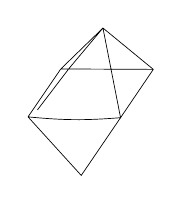
\begin{tikzpicture}[x=.52cm,y=.52cm,line width=.25pt]
\coordinate (a) at (0,0);\coordinate (b) at (1.30,-1.43);\coordinate (c) at (2.26,-.02);
\coordinate (d) at (3.06,1.16);\coordinate (e) at (1.83,2.17);\coordinate (f) at (.80,1.17);
\draw (a)--(b)--(c)--(d) (a)--(f)--(e)--(d) (a) to[bend right=5] (c) (e)--(c)
(f)--(d) (.23,.17)--(1.00,1.18)--(e);
\end{tikzpicture}}

\[
\begin{aligned}
x,\deleted{x'}&=\lambda e+\mu f & x\wedge e&=\pm\mu & x\wedge f&=\pm\lambda\\
x'&=\lambda'e+\mu'f & x'\wedge e&=\pm\mu' & x'\wedge f&=\pm\lambda'\\
\deleted{x\wedge}\ u&=ae+bf & \text{ops}\quad x&=e+\deleted{\unsure{f}}f & u&=\unsure{\checkmark}\\
&&x'&=e-f\\
x\wedge u&=-a+b &\deleted{\unsure{-a+b|a+b}}\\
x'\wedge u&=+a+b & 2a&=0\quad\underline{\text{ou}}\quad 2b=0 &
\deleted{\underline{\text{si }(a,b)=\Lambda}},\quad b-a,\ b+a&\in\Lambda^*
\end{aligned}
\]
